\chapter{Resultados}
\label{cap:resultados}

Este capítulo apresenta os resultados de pesquisa e de desenvolvimento do GOJ. Os resultados das contagens de problemas dos juízes onlines selecionados e a seleção dos juízes estão na seção \nameref{sec:pesquisa_juizes}; os resultados do desenvolvimento da aplicação e seus devidos módulos se encontram na seção \nameref{sec:modulosDaAplicacao}.

\section{Identificação dos principais juízes online exisitentes}
\label{sec:pesquisa_juizes}

Nessa seção serão abordados resultados do levantamento dos juízes online existentes, o que embasou e motivou a criação de um novo juiz online. Esta seção está dividida em duas subseções: a subseção \nameref{subsec:resultados_selecao_juizes}, que mostra os juízes selecionados para as análises; a subseção \nameref{subsec:funcionalidades}, que apresenta funcionalidades relevantes para o GOJ e a presença delas nos juízes selecionados.

\subsection{Identificação e seleção de juízes online}
\label{subsec:resultados_selecao_juizes}

Foram selecionados 10 juízes onlines com base nos critérios e buscas descritas na Subseção \ref{subsec:selecao_juizes}. Os juízes selecionados foram:

\begin{enumerate}
    \item OnlineJudge
    \item Beecrowd
    \item Sphere Online Judge (SPOJ)
    \item PKU JudgeOnline
    \item CodeChef
    \item Google's Coding Competitions
    \item Hackerearth
    \item Codeforces
    \item Neps Academy 
    \item CodeBench
\end{enumerate}

Para o melhor entendimento do impacto e relevância de cada um dos juízes, foi realizado um levantamento do número de problemas de cada um deles, o que pode indicar o engajamento da comunidade, o tempo da plataforma no ar ou a frequência de atualização dos mantenedores; esse levantamento pode ser observado na Tabela \ref{table:detalhes_juizes}. 

\begin{table}[h]
\centering
\begin{threeparttable}
    \caption{Número de problemas e data das buscas que identificaram os juízes online selecionados}
    
    \label{table:detalhes_juizes}
    \begin{tabular}{lcc}
        \toprule
        \textbf{Juíz online}         & \textbf{Problemas} & \textbf{Consulta} \\
        \midrule
        Online Judge                 & 12 483              & 27/03/2022        \\
        Beecrowd                     & 2 283               & 27/03/2022        \\
        Sphere Online Judge (SPOJ)   & 6 027               & 05/04/2022        \\
        PKU Judge Online             & 3 054               & 05/04/2022        \\
        CodeChef                     & 3 363               & 05/04/2022        \\
        Google's Coding Competitions & 224                & 05/04/2022        \\
        Hackerearth                  & 1 526               & 05/04/2022        \\
        Codeforces                   & 7 642               & 27/03/2022        \\
        Neps Academy                 & 1 069               & 05/04/2022        \\
        CodeBench                    & —                  & 05/04/2022   \\
        \bottomrule
    \end{tabular}
    \medskip
    \begin{tablenotes}
        \centering
        \item Fonte: o Autor
    \end{tablenotes}
\end{threeparttable}
\end{table}

A Tabela \ref{table:detalhes_juizes} mostra uma coluna com o título “Problemas”, a qual indica o número de problemas estimado na Subseção \ref{subsec:selecao_juizes} disponíveis para treino; na coluna ``Consulta'' é registrada a data em que o levantamento foi feito. Na última linha da tabela, o juiz online \textit{“Code Bench”} não possui registro de problemas, pois a plataforma funciona com um sistema de turmas fechadas. Deste modo, não foi possível estimar o número de problemas.

\subsection{Funcionalidades}
\label{subsec:funcionalidades}

Para os juízes selecionados foi realizado um levantamento de funcionalidades consideradas relevantes para o projeto GOJ. O objetivo desse levantamento é apresentar a motivação da criação de um novo juiz online, diante dos vários disponíveis. Para se tornar eficaz, esse novo juiz deve ter como funcionalidades: plataforma em português, visto que o público alvo do sistema é um público falante da língua portuguesa; código aberto, para que possíveis melhorias no sistema sejam efetuadas posteriormente por contribuidores interessados; possibilidade de enviar problemas customizados para a plataforma; poder de inserir tutoriais para as questões, para auxiliar os competidores na resolução posterior.

O Quadro \ref{table:funcionalidades_dos_juizes} apresenta as funcionalidades relevantes para o projeto GOJ na coluna ``Funcionalidade''. As demais colunas listam os juízes por sigla. O Quadro assinala com um ``x'' o juiz que possui a funcionalidade. O nome dos juízes foi abreviado, porém, eles seguem a ordem da Tabela \ref{table:detalhes_juizes} e estão apresentados em nota.

\begin{quadro}
    \caption{Funcionalidades Dos Juízes}
    \centering
    \label{table:funcionalidades_dos_juizes}
    \resizebox{15cm}{!} 
    { 
    \begin{threeparttable}
    \begin{tabular}{|l|c|c|c|c|c|c|c|c|c|c|}
        \hline
        \textbf{Funcionalidade} & \textbf{OJ}\footnotemark & \textbf{BC}\footnotemark & \textbf{SPOJ}\footnotemark & \textbf{PKU}\footnotemark & \textbf{CC}\footnotemark & \textbf{GCC}\footnotemark & \textbf{HH}\footnotemark & \textbf{CF}\footnotemark & \textbf{NA}\footnotemark & \textbf{CB}\footnotemark \\ \hline
        \begin{tabular}[c]{@{}l@{}}Plataforma \\ em português\end{tabular}                 &  & x &  &  &   &   &   &   & x & x  \\ \hline
        Código aberto  &    &    &      &     &    &     &    &    &    &    \\ \hline
        \begin{tabular}[c]{@{}l@{}}Possível enviar\\ problemas\\ customizados\end{tabular} &  & x &  &  &   &   &   & x &   &  \\ \hline
        \begin{tabular}[c]{@{}l@{}}Possui tutoriais \\ dos problemas\end{tabular}          &  &   &  &  & x & x & x & x & x &  \\ \hline
    \end{tabular}
    \medskip
    \begin{tablenotes}
        \centering
        \item Fonte: o Autor
    \end{tablenotes}
    \end{threeparttable}
    }
\end{quadro}

\footnotetext[1]{Online Judge}
\footnotetext[2]{Beecrowd}
\footnotetext[3]{Sphere Online Judge}
\footnotetext[4]{PKU JudgeOnline}
\footnotetext[5]{CodeChef}
\footnotetext[6]{Google's Coding Competitions}
\footnotetext[7]{Hackerearth}
\footnotetext[8]{Codeforces}
\footnotetext[9]{Neps Academy}
\footnotetext[10]{CodeBench}

Conforme dito, ``Plataforma em português'' representa os juízes que possuem o site em português ou suporte para a língua. Os únicos juízes que possuem tal funcionalidade são o \textit{Beecrowd} e o \textit{Neps Academy}. Apesar de outras plataformas possuírem problemas na língua portuguesa, como o \textit{Codeforces} por exemplo, estes problemas não são oficiais, ou seja, foram publicados por usuários na plataforma.  

Já ``Código aberto'' indica os juízes que possuem código aberto para contribuidores externos, como no caso do juiz eletrônico “BOCA”, por exemplo, o que possibilita a contribuição ou cópia do mesmo; porém, dentre os juízes pesquisados, nenhum possui esta funcionalidade. 

``Possível enviar problemas customizados'' é aplicado para juízes que permitem o envio de questões customizadas. Apesar de alguns juízes estarem marcados com essa funcionalidade, não é trivial o envio: é preciso preencher alguns pre-requisitos para enviar problemas ou entrar em contato diretamente com a equipe do site para que as questões sejam aprovadas. Apesar disso, foram marcados as plataformas com essa possibilidade. 

Por fim, ``Possui tutoriais dos problemas'' identifica os juízes com suporte para a adição de tutoriais. Algumas das plataformas não tem esse suporte ou não tem a intenção de ter tutoriais nos problemas, como é o exemplo dos juízes com propostas primariamente educativas, voltados para o uso acadêmico em exercícios e provas. Em geral, as plataformas voltadas para competições e treinos de programação competitiva possuem essa funcionalidade.
 
Conforme mostrado no Quadro \ref{table:funcionalidades_dos_juizes}, nenhum dos juízes selecionados abrange todas as funcionalidades relevantes, sendo que o máximo de abrangência foram 2 funcionalidades em um total de 4, motivando a criação desse novo juiz online, cujo objetivo é implementar todas estas quatro funcionalidades.
 
\section{Módulos do GOJ}
\label{sec:modulosDaAplicacao}

O GOJ foi dividido em 4 partes: o Gamma Judge UI, que representa a interface; Gamma Judge API, que além de ser a API ainda funciona com um \textit{worker}, ou seja, trabalha recebendo e processando informações das submissões;  Gamma Judge Tools, assim denominado por conta do MOJ Tools\footnote{https://github.com/cd-moj/mojtools}, módulo responsável por julgar as submissões; e por fim, o Gamma Judge Admin, que também é uma interface, voltada para a edição dos eventos e problemas.

\subsection{Gamma Judge API}
\label{sec:gammaJudgeApi}

Esse módulo da aplicação foi dividido em 3 partes: \textit{API}, \textit{Infrastructure} e \textit{Workers}. A \textit{API} é responsável por efetuar a comunicação externa da aplicação via \textit{HTTP}; a \textit{Infrastructure} é responsável por concentrar a infraestrutura do sistema, como a comunicação com o banco de dados; e os \textit{Workers} são funções executadas periodicamente — nesse caso, para fazer o acesso com o sistema de filas.

Na Figura \ref{fig:judge_ui_folders} é apresentado o esquema de pastas, cada um dos blocos representa um projeto do \textit{.NET} e a organização das principais pastas ou arquivos. Na Api temos 2 pastas principais: \textit{“Controllers”}, que armazena os \textit{endpoints} expostos, onde é feita a comunicação de outros serviços; e \textit{“Models”}, onde estão as estruturas de algumas requisições. \textit{“Infrastructure”} possui em sua maioria funções para comunicação com o banco de dados; já  \textit{“Workers”}, possui um importante arquivo que faz a comunicação com o sistema de filas e recebe o veredicto das questões julgadas.

\begin{figure}
    \centering
    \caption{Esquema de pastas Gamma Judge API}
    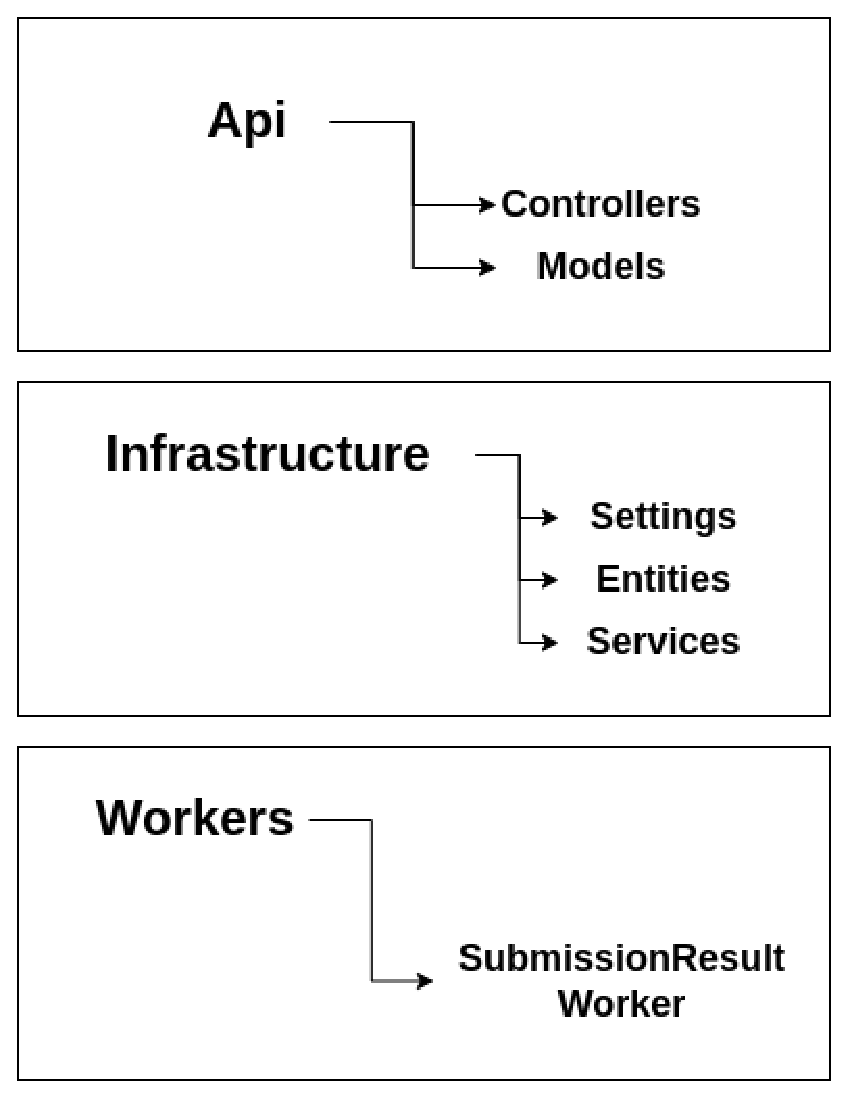
\includegraphics[keepaspectratio=true,scale=0.5]{figuras/gamma_judge_api_folders.eps}
    \label{fig:judge_ui_folders}
    
    \medskip
    Fonte: o Autor
    \medskip
\end{figure}

\subsubsection{Módulo de problemas}
\label{subsubsec:moduloDeProblemas}

O módulo de problemas é responsável pelos problemas e todas as funcionalidades relacionadas às informações expostas para a interface da aplicação. A Figura \ref{fig:problems_endpoints} representa os endereços expostos via API pelo módulo de problemas.

\begin{figure}
    \centering
    \caption{Funções expostas do módulo de problemas}
    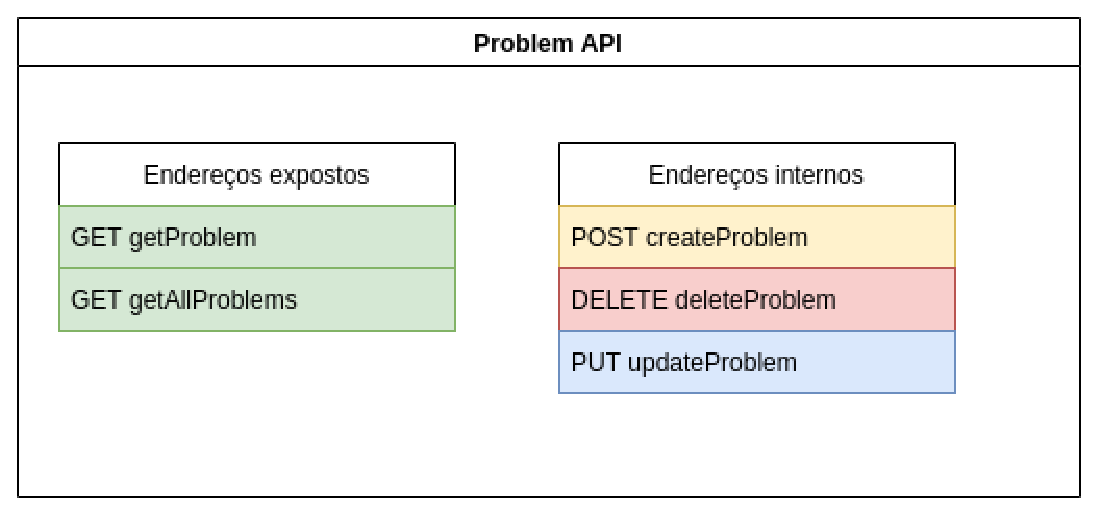
\includegraphics[keepaspectratio=true,scale=0.5]{figuras/problems_endpoins.eps}
    \label{fig:problems_endpoints}
    
    \medskip
    Fonte: o Autor
    \medskip
\end{figure}

A Figura \ref{fig:problems_endpoints} apresenta em ``Endereços expostos'' os endereços que devem ser públicos, acessados pela interface via API; os ``Endereços internos'' listam funções da \textit{API} realizados para uso interno, possibilitando o cadastro, edição e remoção de um problema sem a necessidade da comunicação direta com o banco de dados.

\subsubsection{Módulo de eventos}
\label{subsec:moduloDeEventos}

O módulo de eventos é responsável pelas informações expostas relacionadas aos eventos cadastrados no banco de dados. A Figura \ref{fig:contests_endpoint} exemplifica o funcionamento desse módulo da API.

\begin{figure}
    \centering
    \caption{Funções expostas do módulo de eventos}
    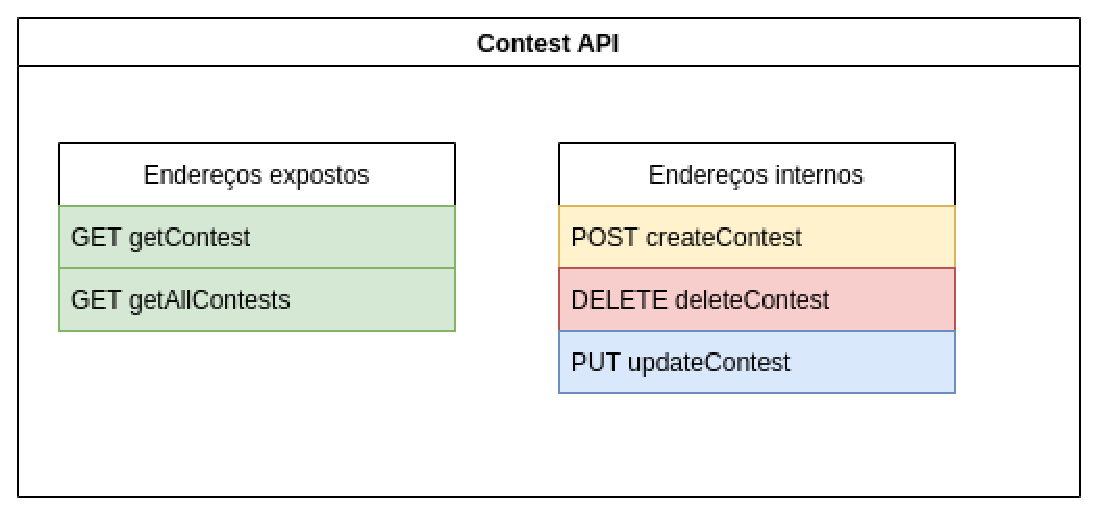
\includegraphics[keepaspectratio=true,scale=0.5]{figuras/contests_endpoint.eps}
    \label{fig:contests_endpoint}
    
    \medskip
    Fonte: o Autor
    \medskip
\end{figure}

O comportamento desse módulo é similar ao do módulo de problemas (Subseção \ref{subsubsec:moduloDeProblemas}). Ele expõe endereços internos, compostos por funções de criação, edição e remoção de eventos. Além disso, são disponibilizadas funções para recuperação de um único evento ou de vários eventos.

\subsection{Gamma Judge UI}
\label{sec:gamaJudgeUI}

A interface do GOJ é um site, com páginas que apresentam as questões e os eventos. O objetivo da interface é organizar as informações da API para o usuário e permitir as submissões. O site pode ser dividido em 2 diferentes módulos: ``Questões'', que representa as páginas que apresentam informações sobre os problemas cadastrados na plataforma; e ``Eventos'', com as páginas responsáveis por exibir as informações sobre os eventos. 

% A interface de usuário se concentra em um site. A aplicação tem o foco de ser simples e possuir módulos facilmente editáveis e substituíveis. Com base nisso a ferramenta de desenvolvimento da interface foi o \textit{React} \cite{rawat2020react}, utilizando \textit{Typescript} \cite{richards_et_al:CTTS} como linguagem principal.

% A ideia da interface ser dividida em componentes, visa a reutilização dos mesmos. Atualmente existem várias aplicações para juízes online, eles podem ser utilizados para o aprendizado em disciplinas de programação \cite{francisco2016juiz}, podem ser utilizados para competições de programação \cite{halim2013competitive} ou para armazenar questões de eventos, como funciona hoje no site da Olimpíada brasileira de informática \cite{obi2021}.

% Com a arquitetura e componentes divididos a interface pode ser adaptada para outras aplicações. A arquitetura em micro serviços permite futuramente que essa aplicação seja usada para outros fins de maneira mais fácil \ref{sec:microServicos}.
% TODO -- Ver o que fazer com o texto comentado 

\subsubsection{Questões}

O módulo de questões da interface é responsável por disponibilizar ao usuário as informações a respeito das questões. Os dados disponíveis aqui são referentes aos dados da Subseção \ref{subsubsec:moduloDeProblemas}. Na Figura \ref{fig:question3} é possível observar a organização e a maneira com que os dados são disponibilizados ao usuário.

\begin{figure}
    \centering
    \caption{Interface - informações da questão}
    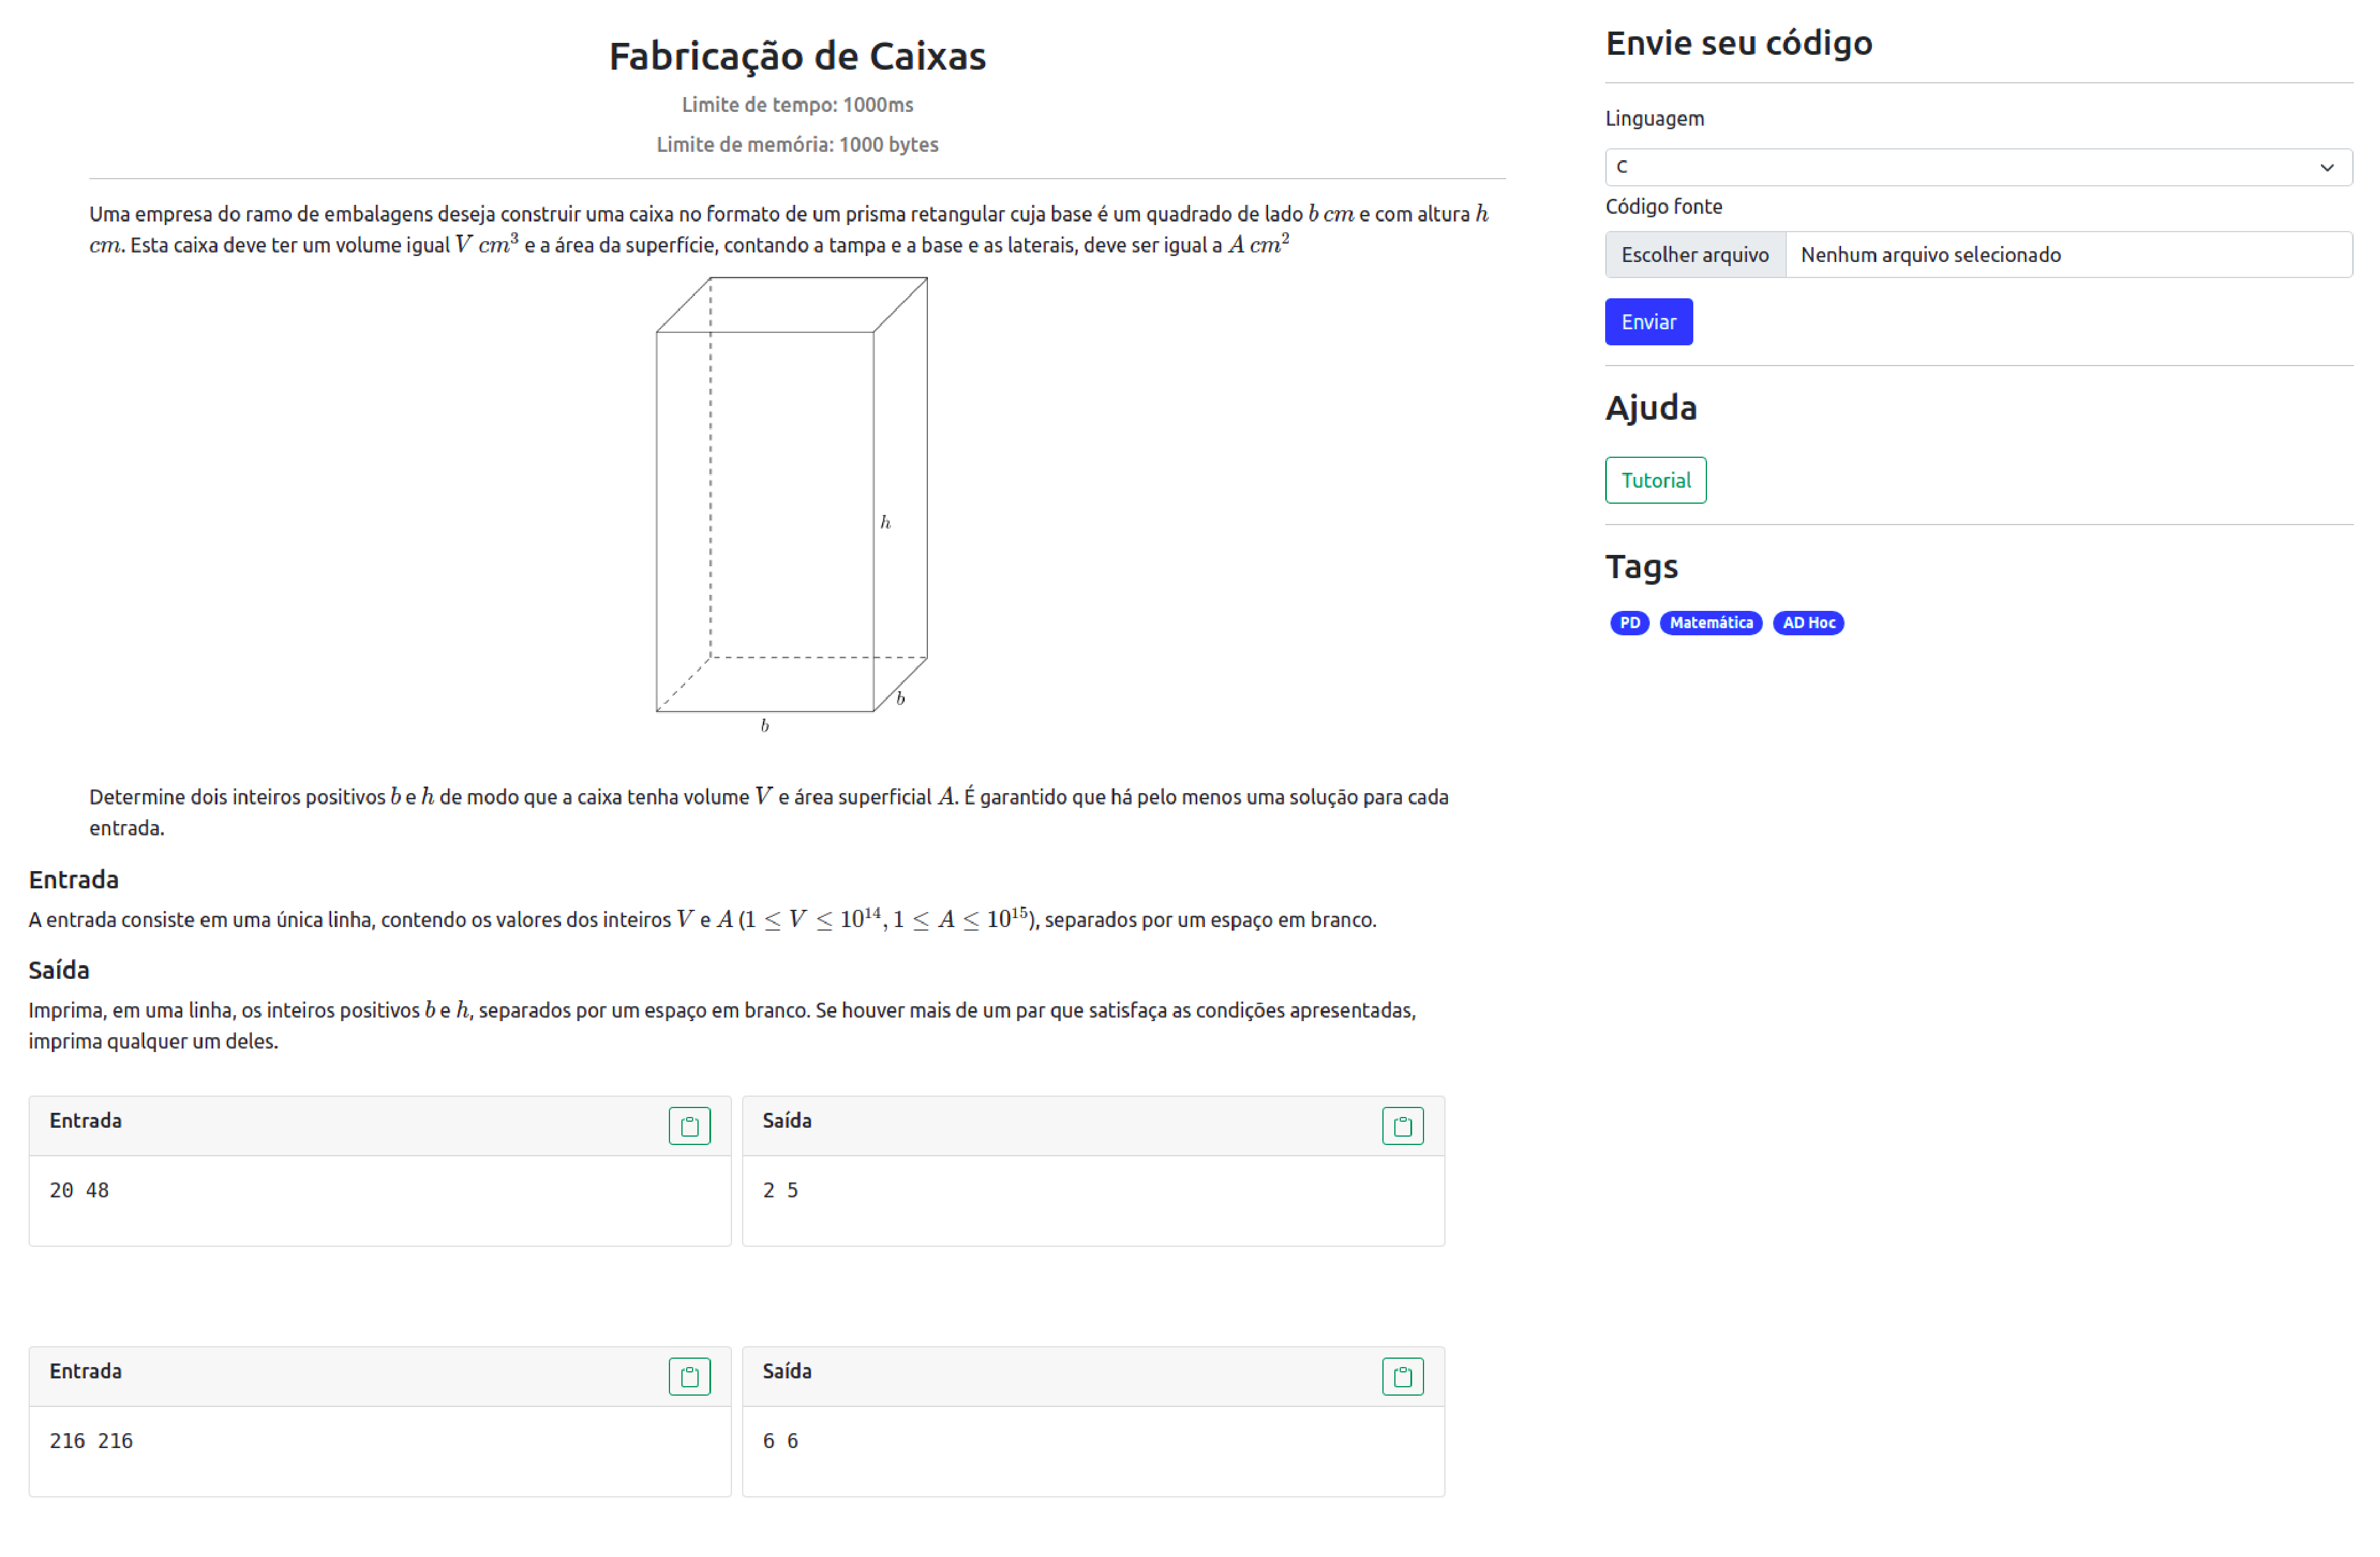
\includegraphics[keepaspectratio=true,scale=0.2]{figuras/question3.eps}
    \label{fig:question3}
    
    \medskip
    Fonte: o Autor
    \medskip
\end{figure}

A interface das questões é dividida em algumas partes: o menu lateral, observável na Figura \ref{fig:sendQuestion1}; as entradas e saídas, disponíveis na Figura \ref{fig:questionInputs}; e o enunciado, disponível na Figura \ref{fig:questionStatement2}.


\begin{figure}[H]
    \centering
    \caption{Interface — envio de questão}
    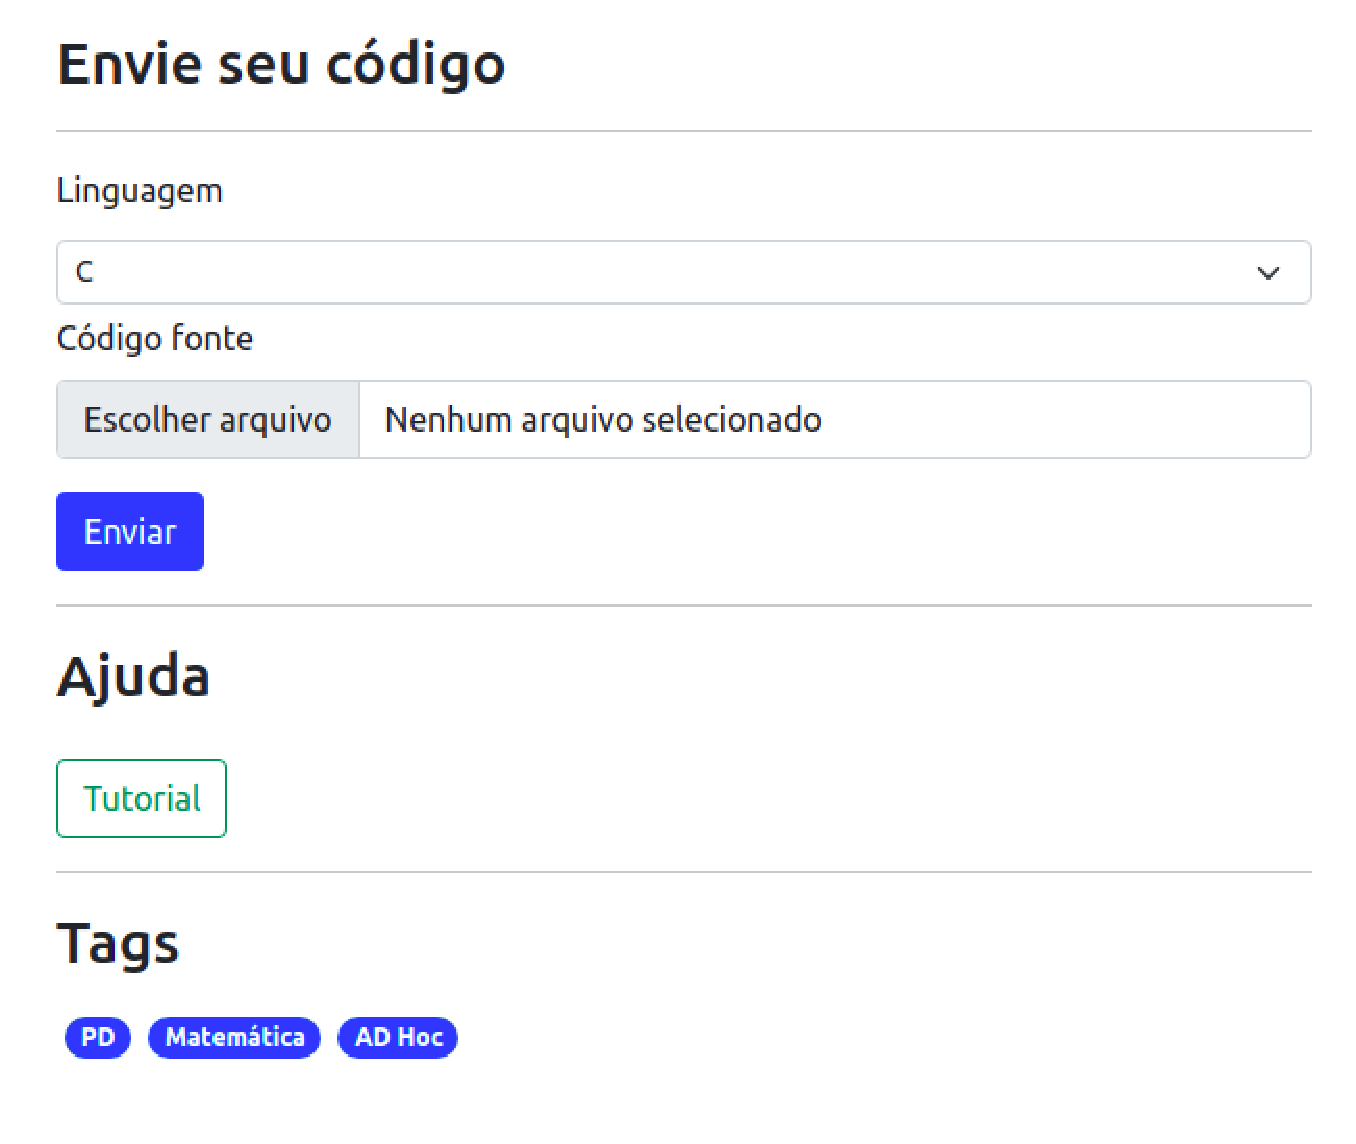
\includegraphics[keepaspectratio=true,scale=0.5]{figuras/sendQuestion1.eps}
    \label{fig:sendQuestion1}
    
    \medskip
    Fonte: o Autor
    \medskip
\end{figure}
    
\begin{figure}[H]
    \centering
    \caption{Interface — entradas e saídas da questão}
    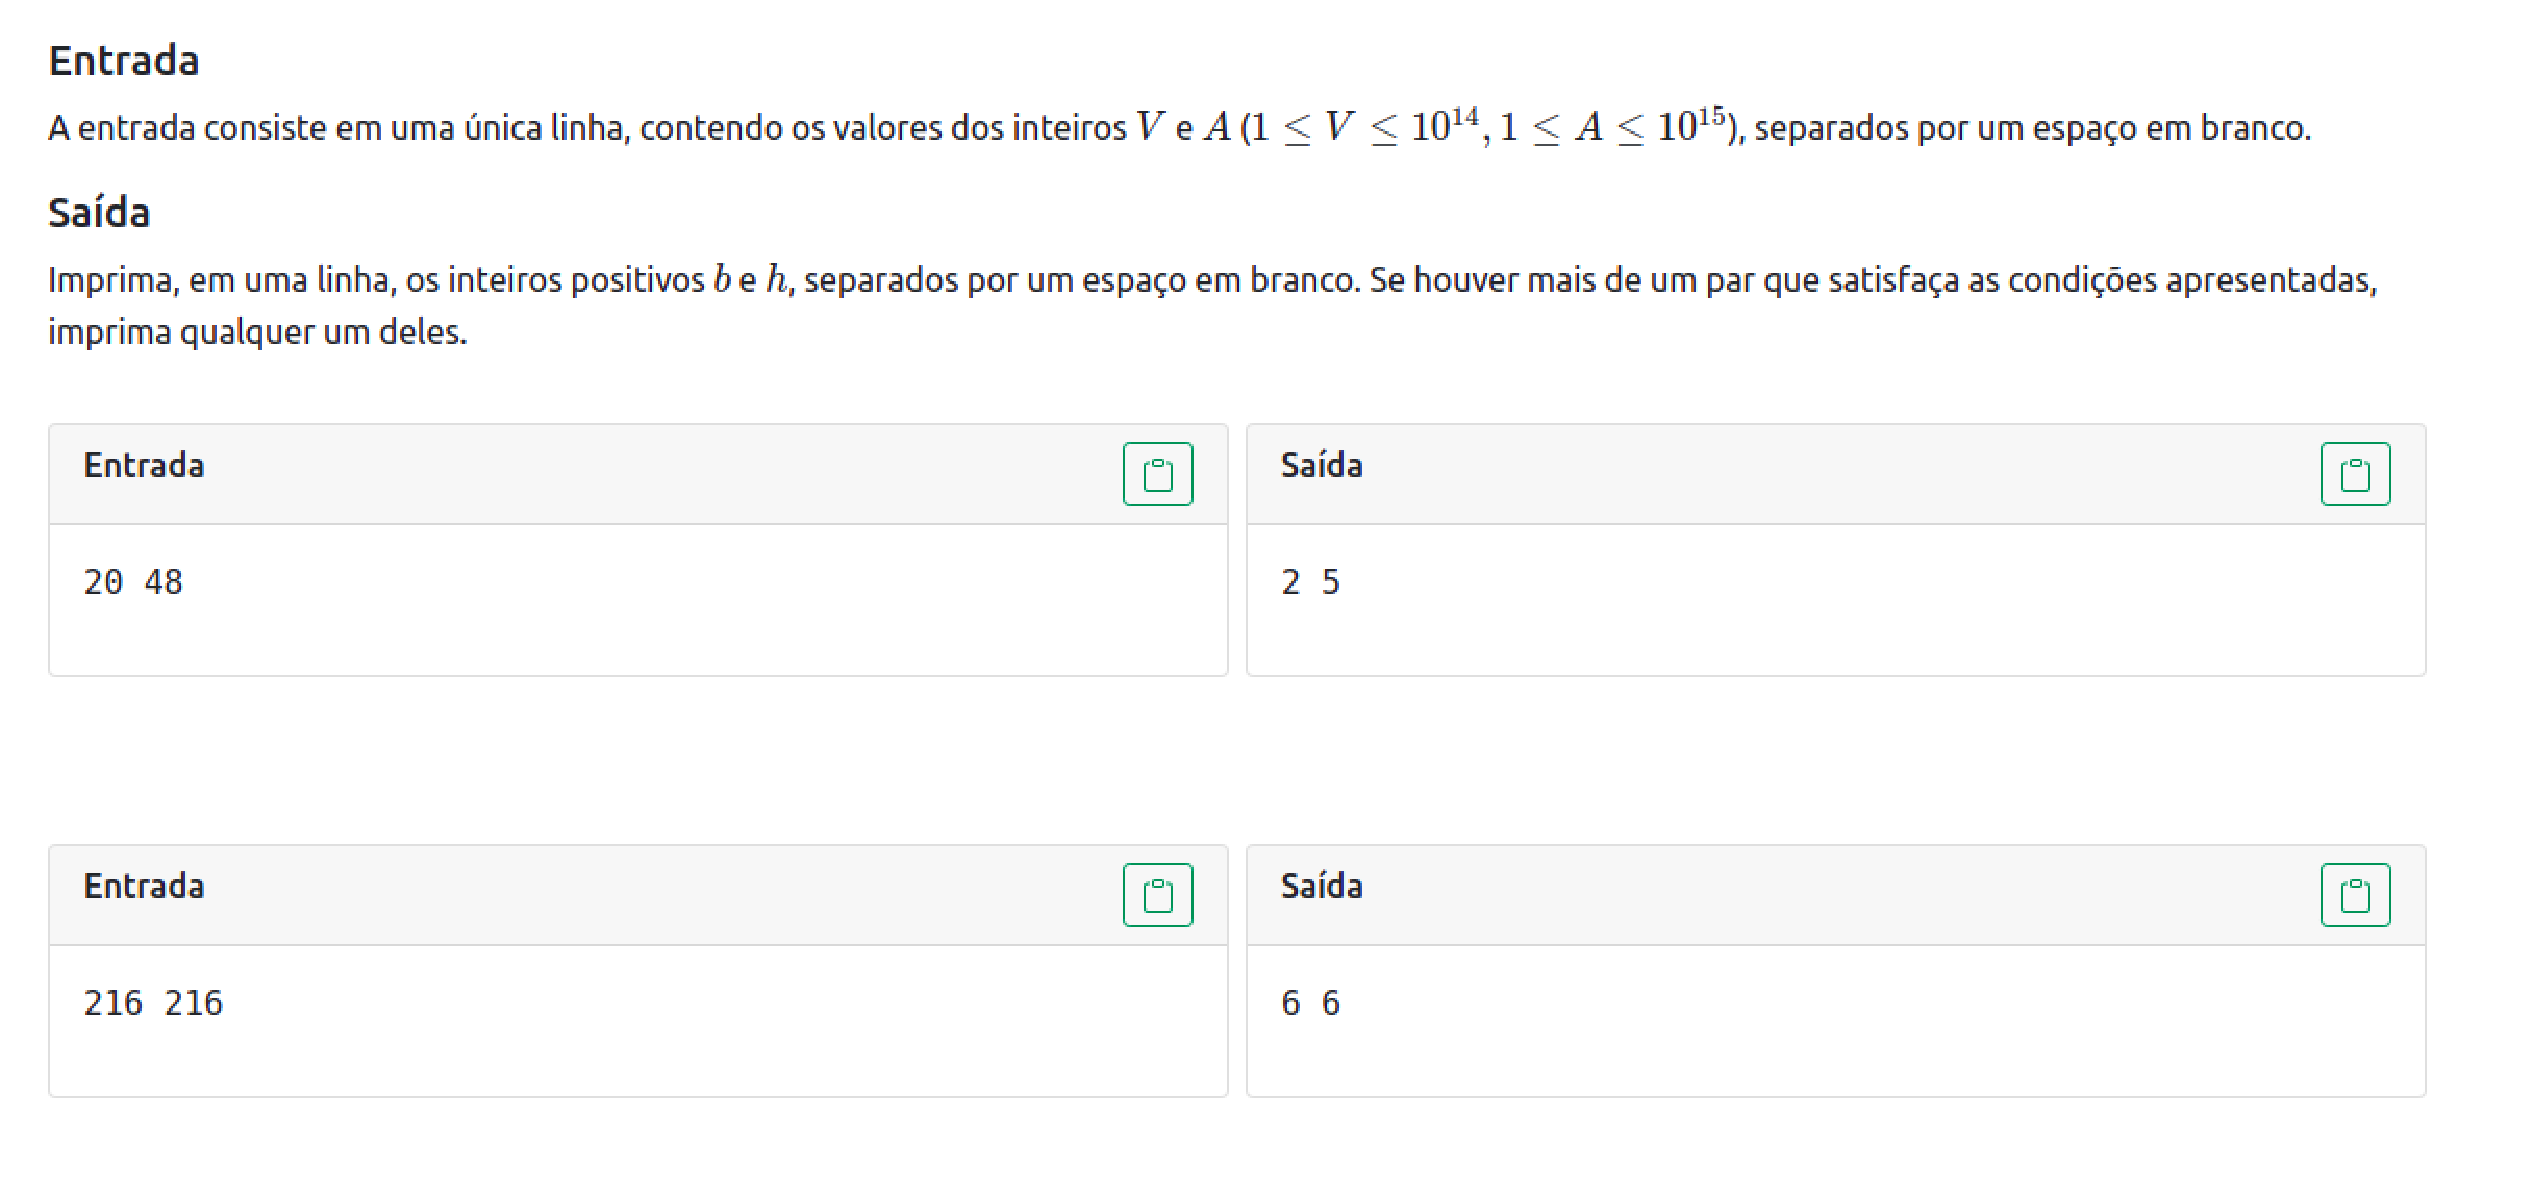
\includegraphics[keepaspectratio=true,scale=0.35]{figuras/questionInputs.eps}
    \label{fig:questionInputs}
    
    \medskip
    Fonte: o Autor
    \medskip
\end{figure}

\begin{figure}[H]
    \centering
    \caption{Interface — Enunciado da questão}
    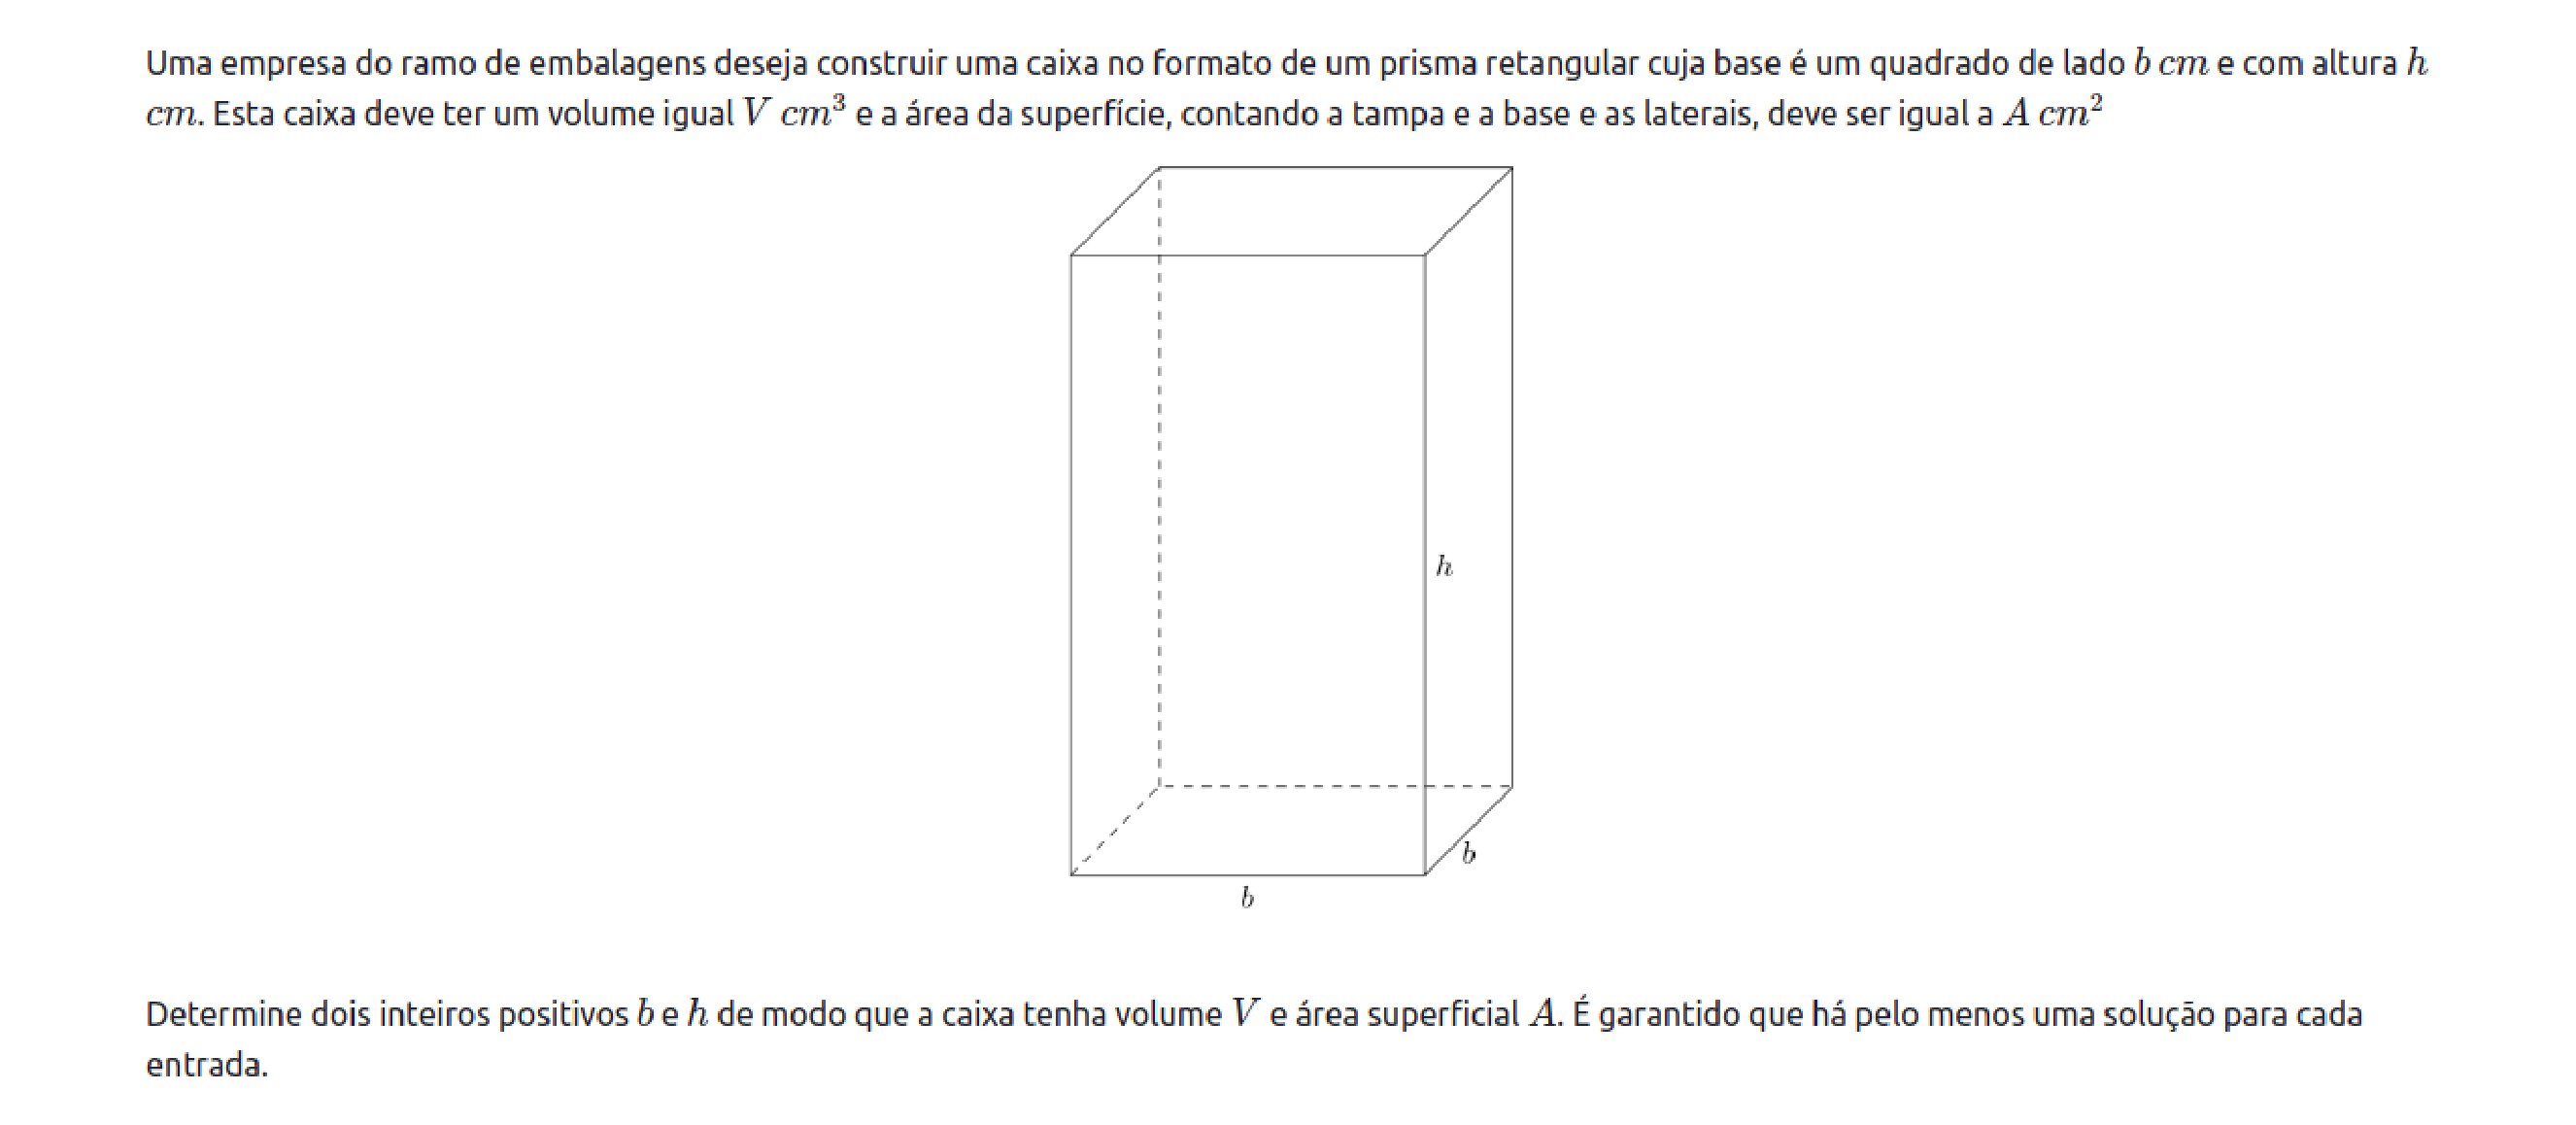
\includegraphics[keepaspectratio=true,scale=0.35]{figuras/questionStatement2.eps}
    \label{fig:questionStatement2}
    
    \medskip
    Fonte: o Autor
    \medskip
\end{figure}

Em juízes online, elementos não textuais são usados para dar mais riquezas e detalhes aos problemas. Assim sendo, é comum a utilização de imagens, fórmulas matemáticas e elementos para enfatizar trechos dos problemas, como textos em negrito ou itálico. Além de apresentar as informações do problema, a interface também é responsável por representar elementos da API\footnote{Ver em \ref{subsec:arquitetura_judge_ui}}, em HTML\footnote{RAGGETT, Dave et al. HTML 4.01 Specification. W3C recommendation, v. 24, 1999.}  ou \LaTeX\footnote{LAMPORT, Leslie. LaTeX. Company Cyfronet, 1991.}, em elementos não textuais; a Figura \ref{fig:questionStatement} exemplifica a utilização desses recursos.

\begin{figure}
    \centering
    \caption{Interface -- demonstração de elementos não textuais}

    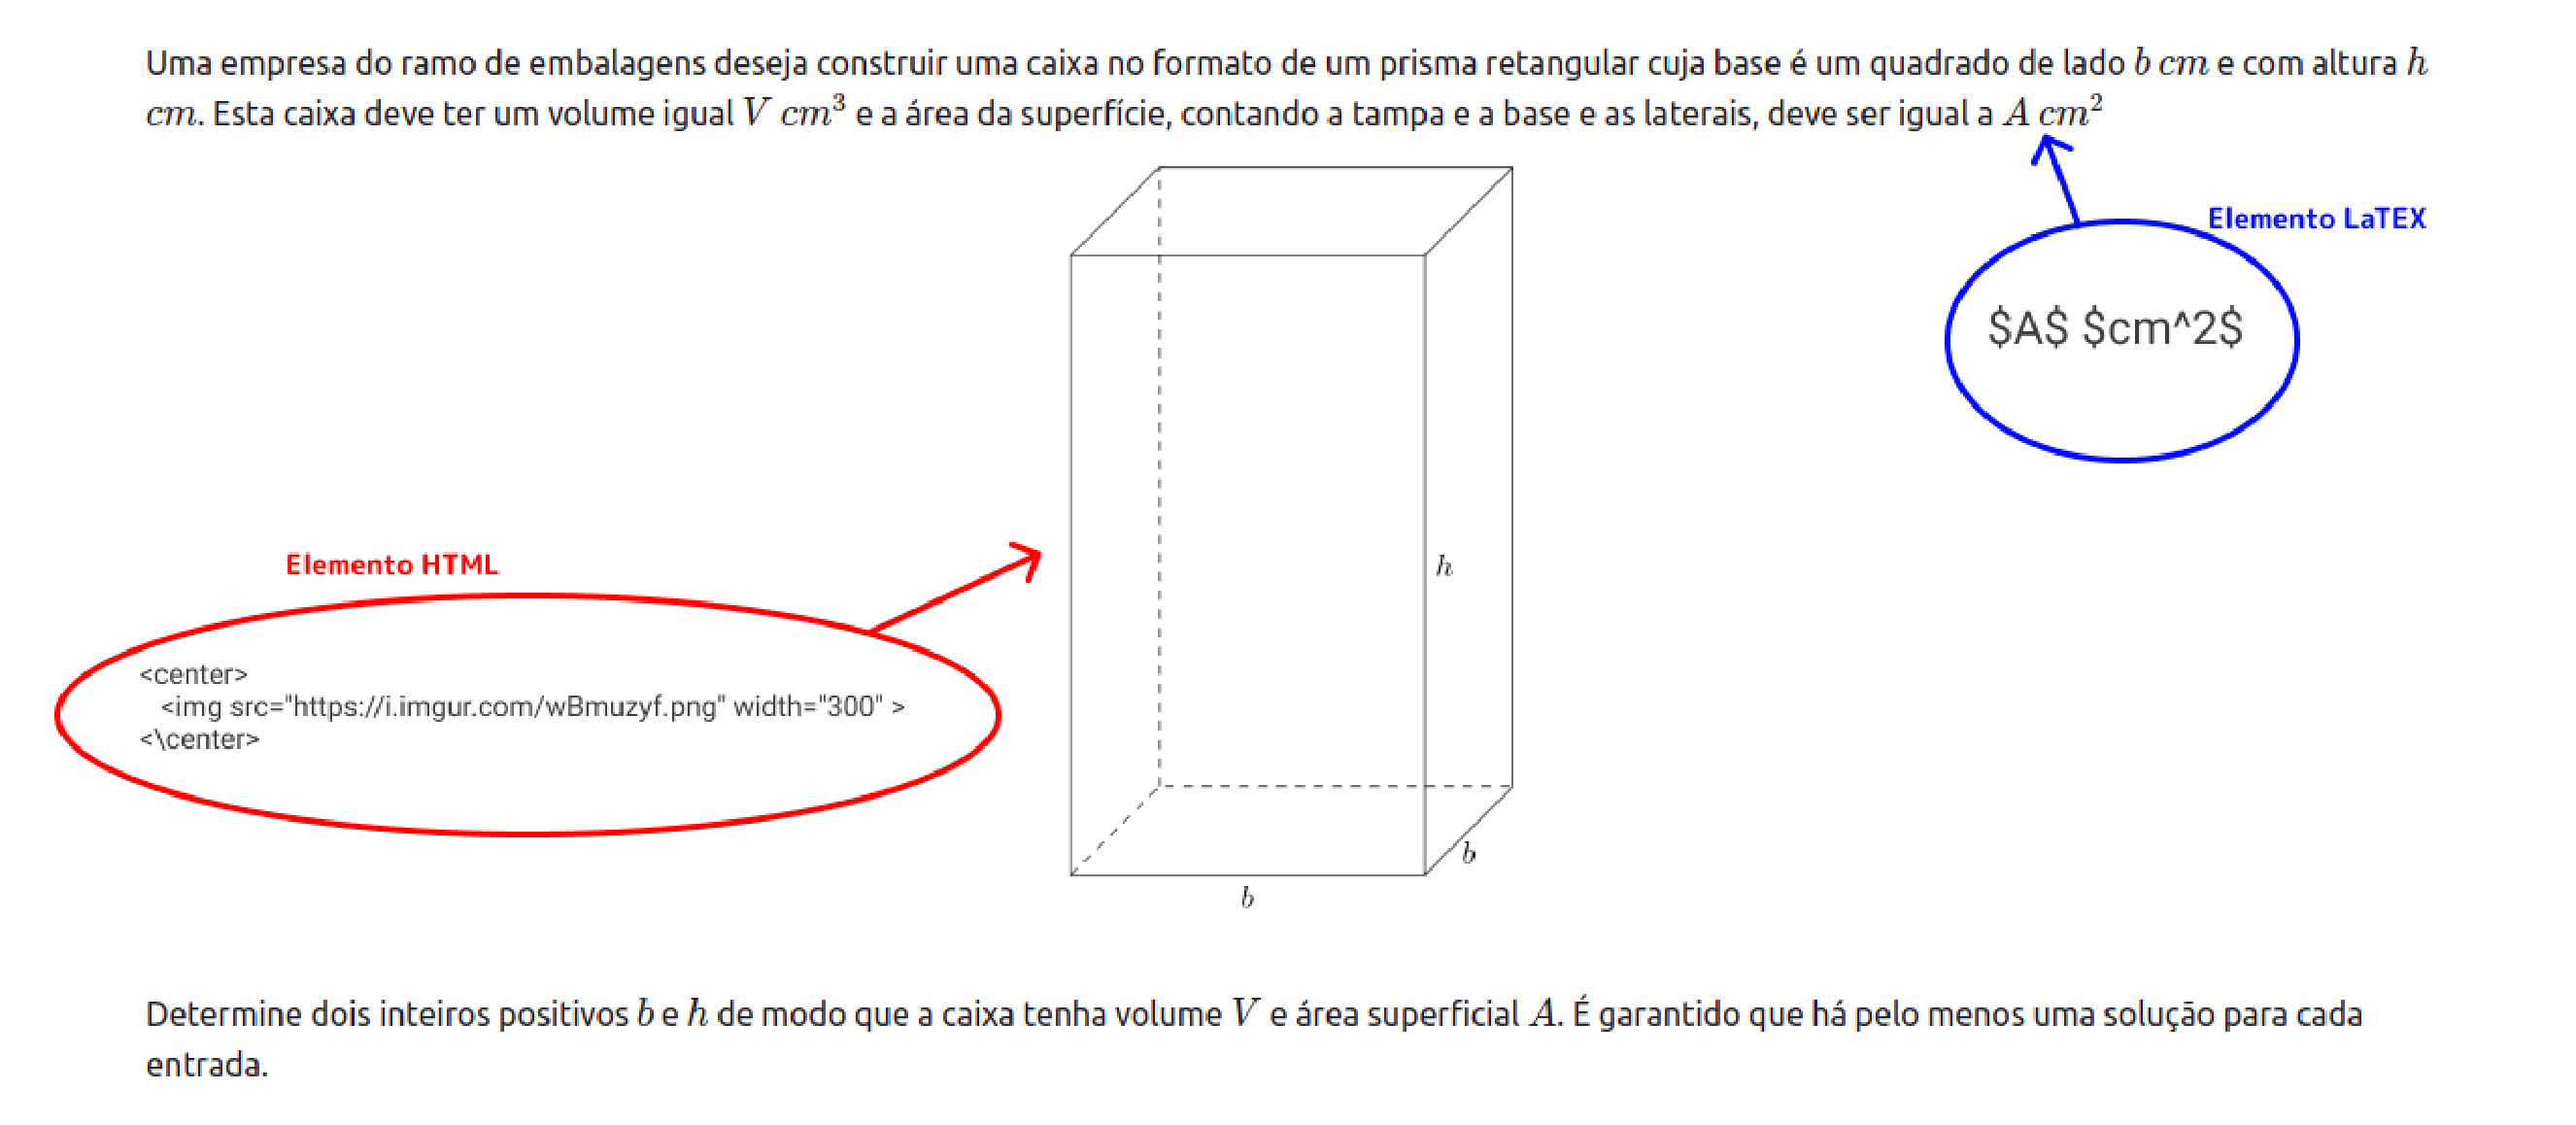
\includegraphics[keepaspectratio=true,scale=0.35]{figuras/questionStatement.eps}
    \label{fig:questionStatement}
    
    \medskip
    Fonte: o Autor
    \medskip
\end{figure}

A Figura \ref{fig:questionStatement} foi renderizada automaticamente a partir de um texto plano vindo da API. O texto utilizado está disponível na Figura \ref{fig:statementText}, tal como o resultado da sua renderização realizada pela aplicação, disponível na Figura \ref{fig:questionStatement2}. Como apresentado na Figura \ref{fig:questionStatement}, neste enunciado foram utilizados elementos da linguagem \LaTeX em azul e elementos HTML em vermelho.

\begin{figure}[H]
    \centering
    \caption{Texto bruto enunciado}
    
\includegraphics[keepaspectratio=true,scale=0.65]{figuras/statementText.eps}
    \label{fig:statementText}

    \medskip
    Fonte: o Autor
    \medskip
\end{figure}

\subsubsection{Eventos}
\label{subsec:eventos}

O módulo de eventos concentra as informações referentes a um determinado evento da Maratona UnB de Programação. Nesse módulo está concentrada a lista de questões do evento e a data em que o evento ocorreu. Os problemas de um evento podem ser reaproveitados em outros, portanto, também é apresentado a origem do problema, que pode ser original do evento ou apresentar onde ele teve origem. A Figura \ref{fig:maratonaUnB} mostra a maneira que as informações são disponibilizadas ao usuário na tela.

\begin{figure}
    \centering
    \caption{Interface -- Detalhes de um evento}
    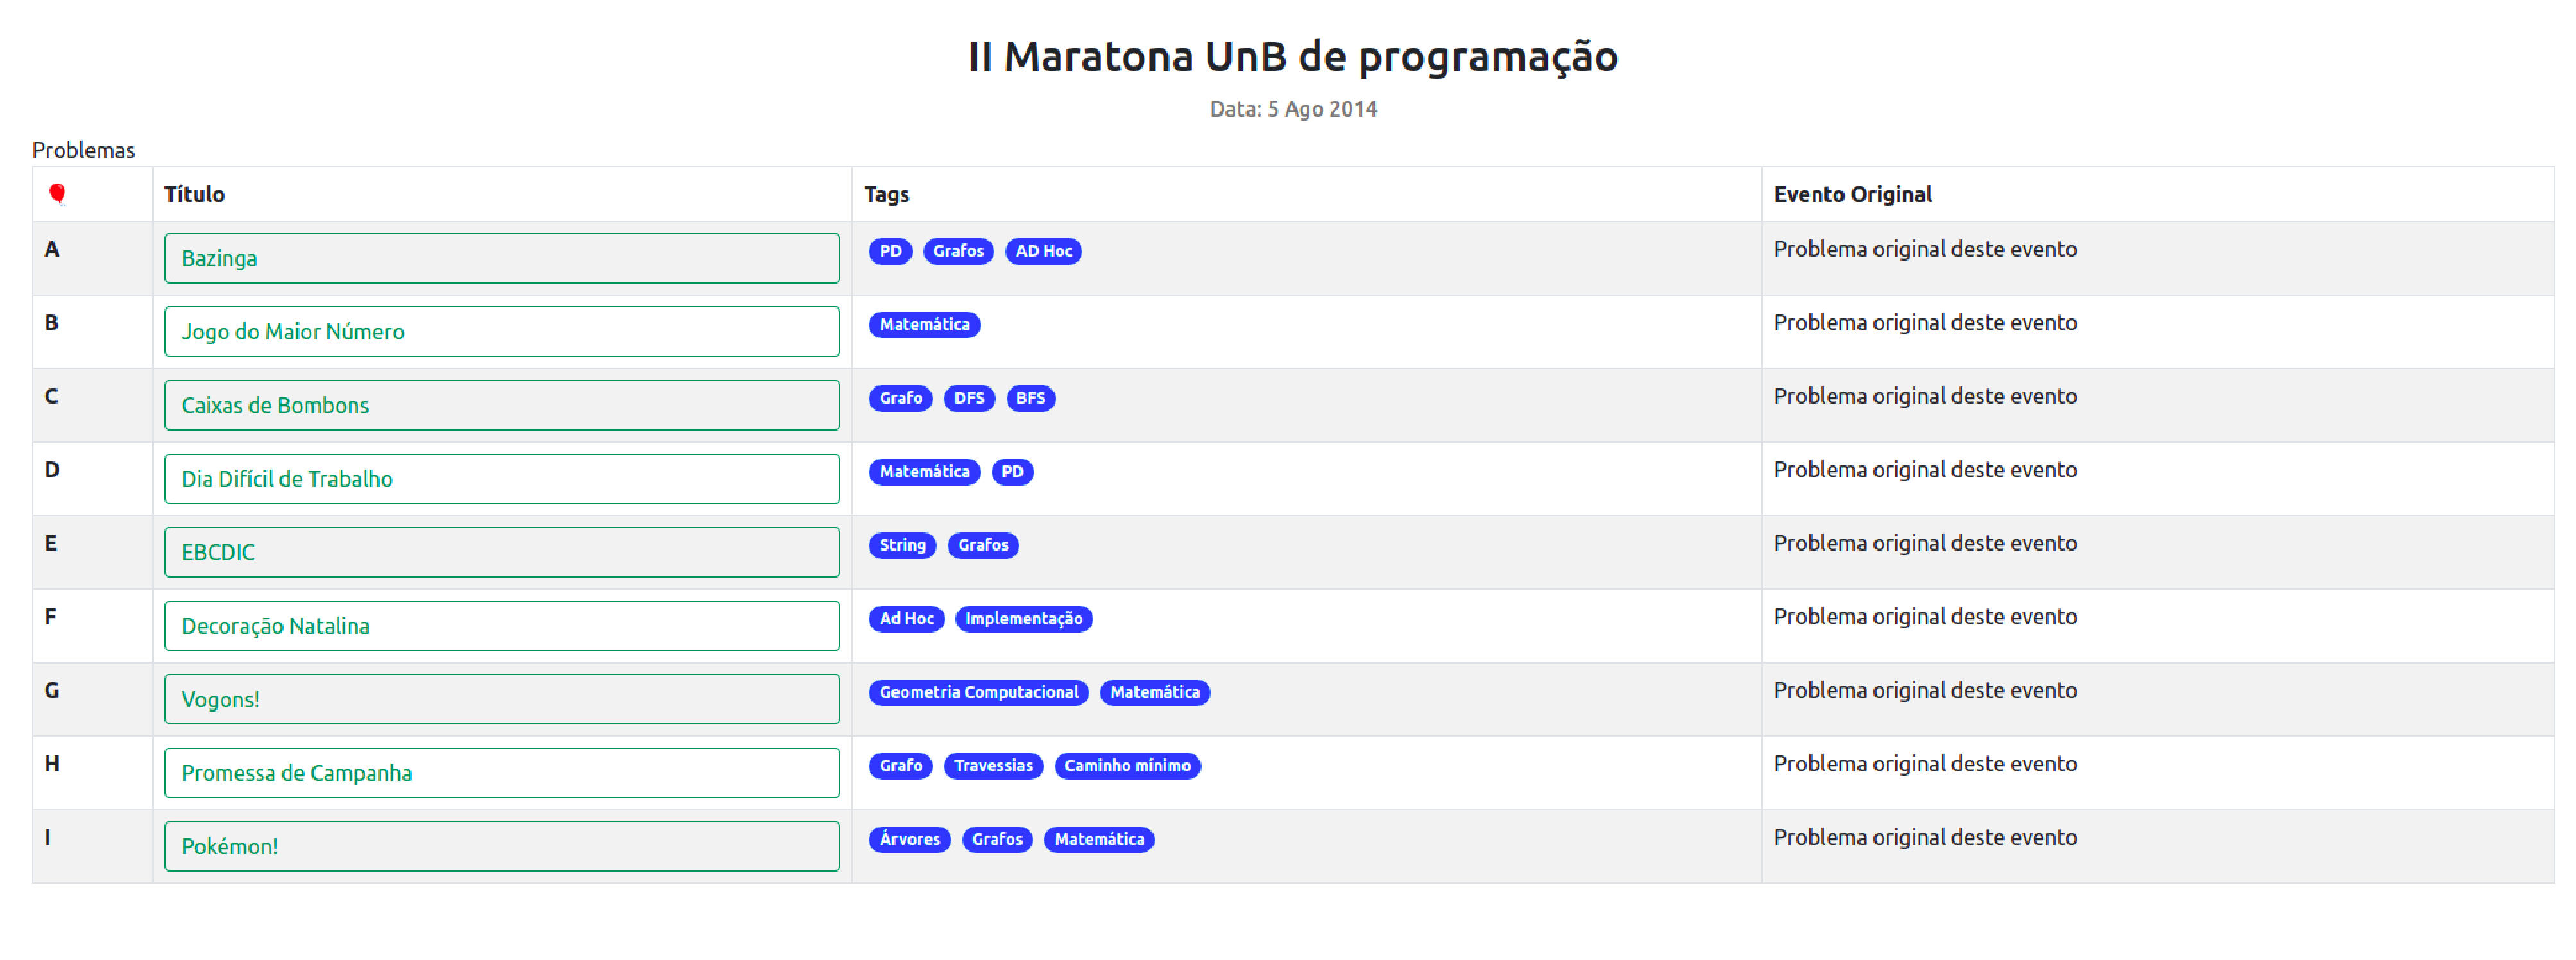
\includegraphics[keepaspectratio=true,scale=0.23]{figuras/contest2.eps}
    \label{fig:maratonaUnB}
    
    \medskip
    Fonte: o Autor
    \medskip
\end{figure}


Como apresentado na Figura \ref{fig:maratonaUnB}, são disponibilizadas informações do rótulo do problema\footnote{O rótulo é representado na Figura \ref{fig:maratonaUnB} com um ícone de balão.}, título, marcações\footnote{As marcações são representadas na Figura \ref{fig:maratonaUnB} como \textit{tags}.} e o evento original da questão. Diferentemente do que mostra a Figura \ref{fig:maratonaUnB}, é possível que nos eventos os problemas sejam marcados com rótulos diferentes das letras do alfabeto. Além disso, o campo ``Evento original'' pode mostrar um botão para o evento em que aquele problema foi criado, caso ele tenha sido reaproveitado nessa maratona.

\subsection{Gamma Judge Tools}
\label{sec:gamaJudgeTools}

Essa parte do sistema é responsável por julgar as submissões enviadas e retornar o veredito; para isso foi utilizada a ferramenta de código aberto MOJ Tools\footnote{https://github.com/cd-moj/mojtools}, responsável por compilar o código recebido, gerar um programa executável, e executá-lo em uma lista de testes (Seção \ref{sec:juizesOnline}).

\begin{figure}
    \centering
    \caption{Gamma judge tools -- Diagrama}
    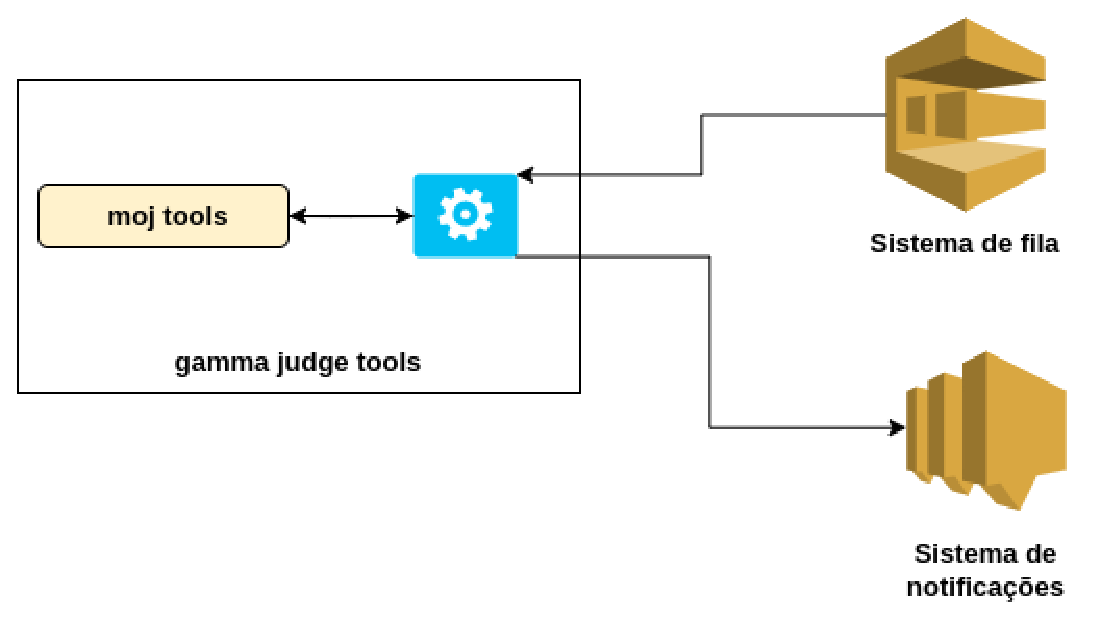
\includegraphics[keepaspectratio=true,scale=0.5]{figuras/gamma_judge_tools_diagram.eps}
    \label{fig:judge_tools_diagram}
    
    \medskip
    Fonte: o Autor
    \medskip
\end{figure}

Na Figura \ref{fig:judge_tools_diagram}, o GOJ lê do sistema de filas uma mensagem contendo as informações da submissão. Após o uso do MOJ Tools para julgar, o veredito é retornado para um sistema de notificações; com isso, as outras aplicações são responsáveis por lidar com a notificação enviada e processar o veredito da submissão. 

\subsection{Gamma Judge Admin}
\label{sec:gamaJudgeAdmin}

O módulo \textit{Gamma Judge Admin} permite o uso de funções de leitura e escrita da API, com mecanismos para ler, criar, editar e deletar um evento ou um problema. Esse módulo permite a manutenção e edição do conteúdo dos problemas armazenados. Sua estrutura se divide em 3 páginas:\textit{ “HomePage”}, que possui apenas botões para as outras páginas; \textit{``ProblemPage''}, que possui os mecanismos descritos, direcionados para os problemas; e \textit{``ContestPage''}, que se assemelha à \textit{``ProblemPage''}, porém direcionada para eventos.

\subsubsection{Problem Page}

A pagina de problemas acessa a API apresentada na Subseção \ref{sec:gammaJudgeApi}, que tem como base o \textit{customId}, uma sequência de caracteres que identifica cada um dos problemas unicamente. A Figura \ref{fig:judge_admin_problem} ilustra a página descrita: com o botão \textit{``GET''}, em verde, e o \textit{customId} preenchido, é possível recuperar as informações de um problema; \textit{``PUT''}, em azul, cria, caso não exista, ou sobrescreve as informações do problema; \textit{``DELETE''}, em vermelho, apaga o problema.

\begin{figure}
    \centering
    \caption{Gamma judge Admin -- ProblemPage}
    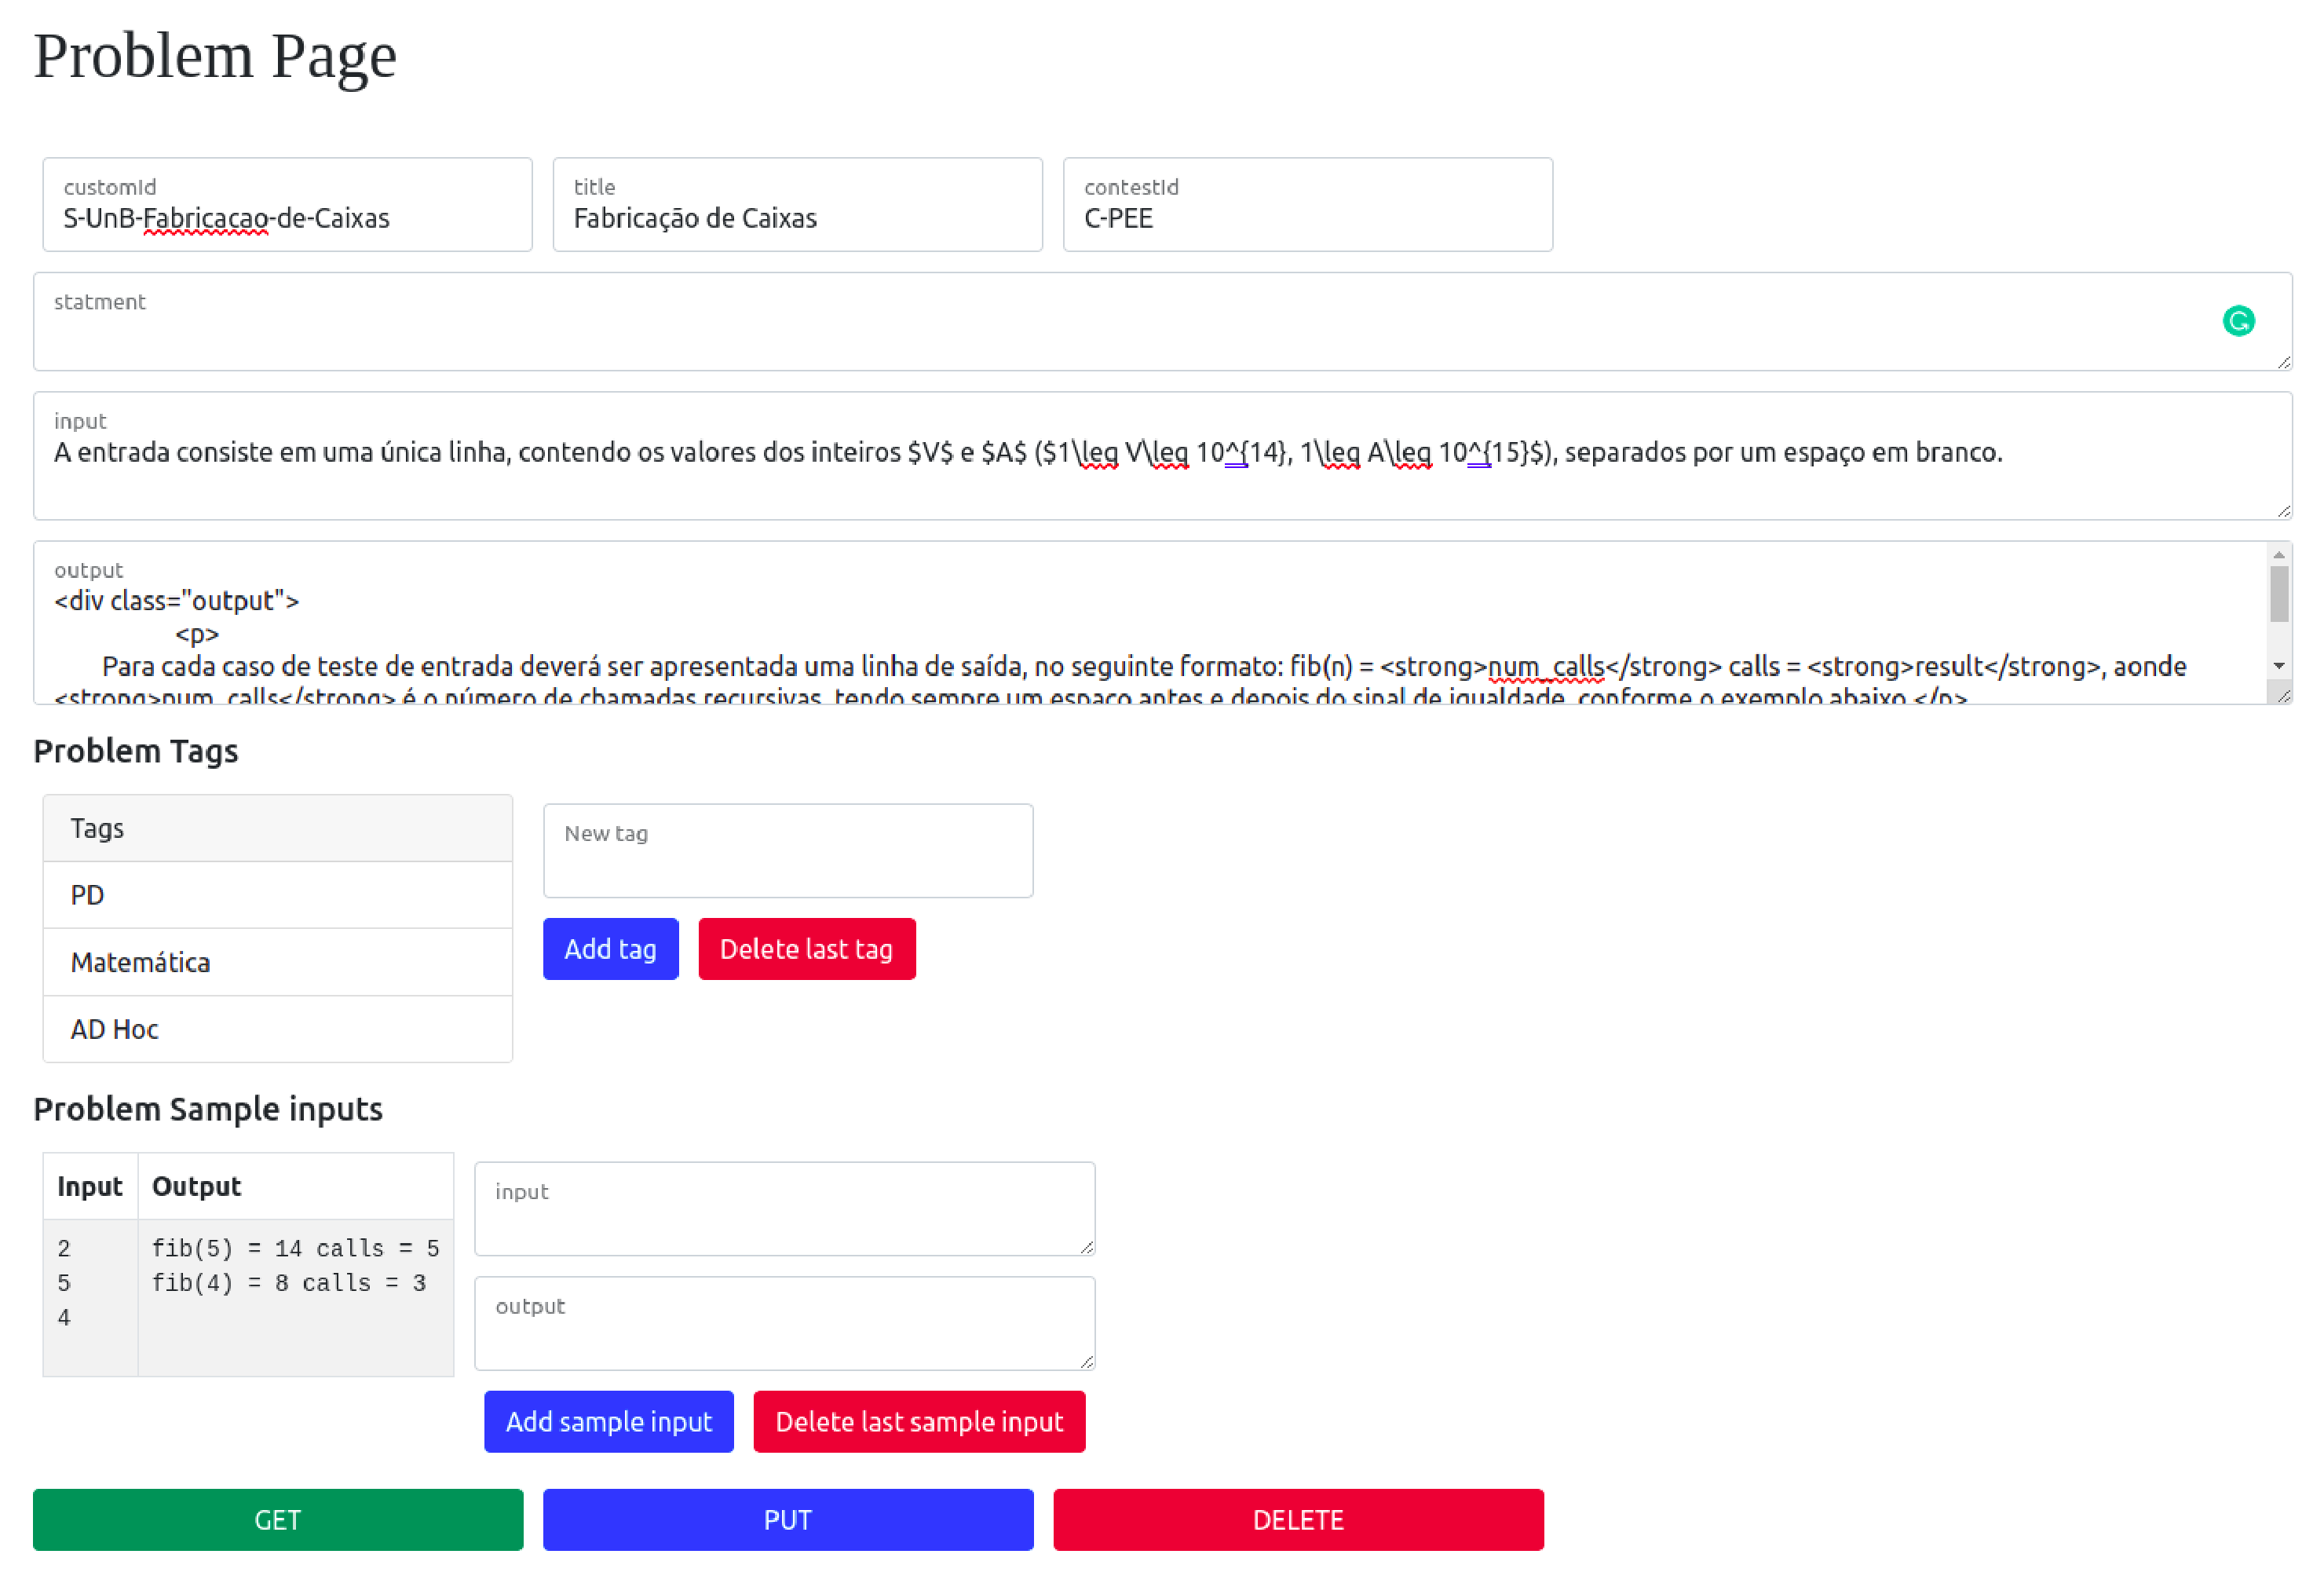
\includegraphics[keepaspectratio=true,scale=0.32]{figuras/problem_page.eps}
    \label{fig:judge_admin_problem}
    
    \medskip
    Fonte: o Autor
    \medskip
\end{figure}

\subsubsection{Contest Page}

A página de eventos tem o comportamento similar à página de problemas, com os mesmos botões e mesmo funcionamento, porém com menos informações. Na página de eventos é possível adicionar ou remover problemas ao evento utilizando o \textit{customId} do problema e o \textit{identifier} será o identificador do problema naquele evento, como mostra a Figura \ref{fig:judge_admin_contest}.

\begin{figure}
    \centering
    \caption{Gamma judge Admin -- ContestPage}
    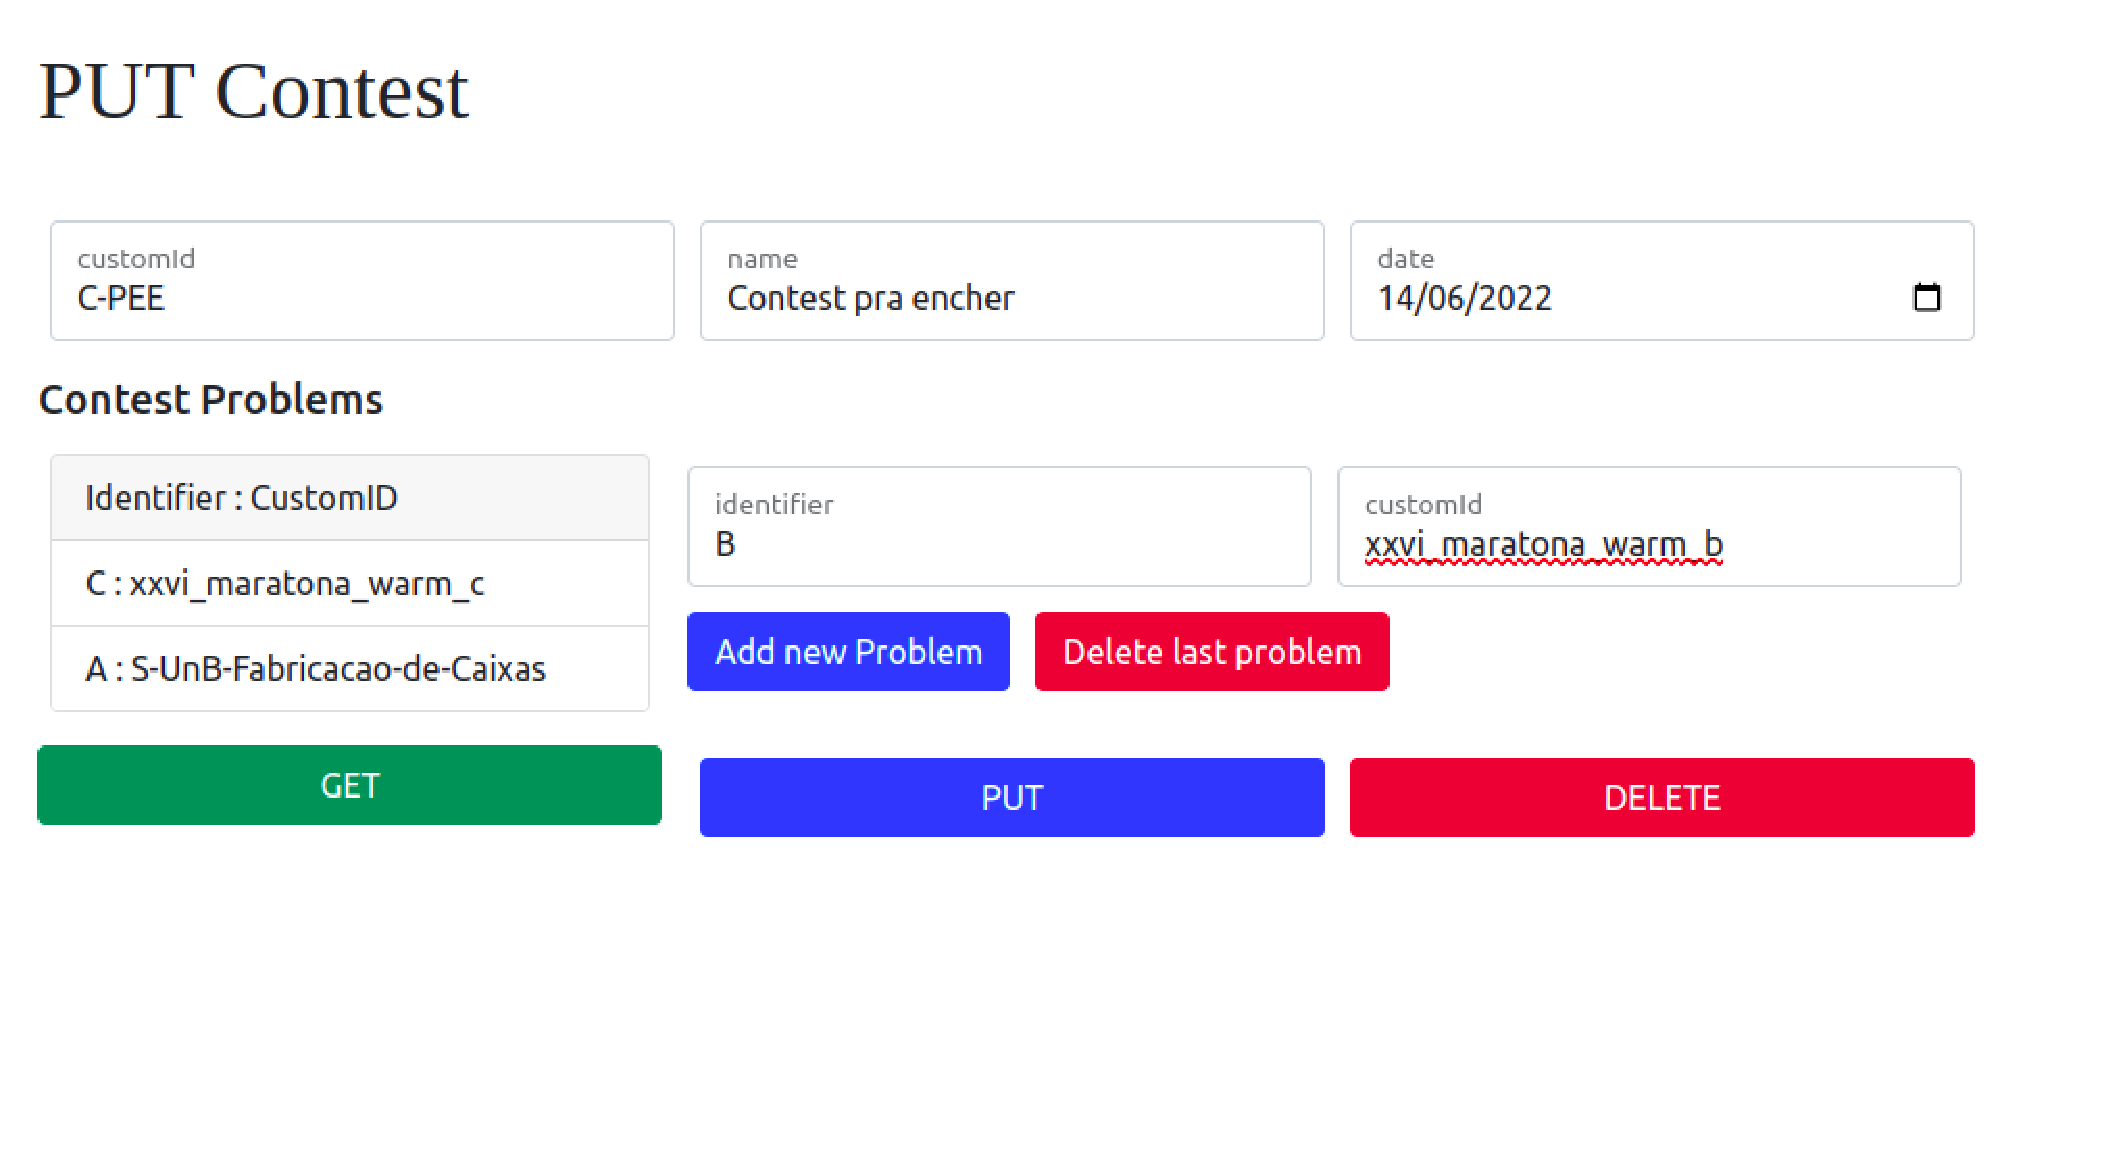
\includegraphics[keepaspectratio=true,scale=0.45]{figuras/contest_page.eps}
    \label{fig:judge_admin_contest}
    
    \medskip
    Fonte: o Autor
    \medskip
\end{figure}
Conforme descrito, a ferramenta possui as funcionalidades almejadas, apresentadas na subseção \ref{subsec:funcionalidades}, possibilitando a sua utilização para armazenamento das questões das Maratonas UnB de Programação. Com isso, o GOJ provê as funcionalidades não observadas nos juízes online pesquisados, fato que justifica seu desenvolvimento e adoção.
